% !TEX program = pdflatex -> bibtex -> pdflatex*2
\documentclass[en]{assignment}
\ProjectInfos*{Quantum Mechanics}{PHYS1501}{Fall, 2020}{Assignment 1}{Due date :2020. 09. 08 (Tuesday)}{Multipluz}{45875852}

\begin{document}
    \begin{prob}
        Show that this \LaTeX template support following functions:
        \begin{itemize}
            \item[(1)] Mathematical formulas;
            \item[(2)] Chemistry formulas.
        \end{itemize}
    \end{prob}
    \begin{sol}
        \begin{itemize}
            \item[(1)] In three-dimensional space, the Schrödinger equation of a particle in a potential $V(\bm{r},t)$ is
            \begin{equation}
                i\hbar\frac{\partial}{\partial t}\ket{\psi(\bm{r},t)}=-\frac{\hbar^2}{2m}\nabla^2\ket{\psi(\bm{r},t)}+V(\bm{r},t)\ket{\psi(\bm{r},t)}.
            \end{equation}
            \item[(2)] Heating and using concentrated sulfuric acid as catalyst, benzene can react with nitric acid to produce nitrobenzene:
            % online tool: https://py-chemist.com/mol_2_chemfig/home
            \begin{equation}
                \ce{\chemfig{*6([,.5]-=-=-=)} + \chemfig{[,.75]HO-NO_2} ->[\mbox{concentrated }H2SO4][$\Delta$] \chemfig{*6([,.5]-=-(-NO_2)=-=)} + H2O}
            \end{equation}
        \end{itemize}
    \end{sol}

    \clearpage

    \begin{prob}
        Conduct following operation:
        \begin{itemize}
            \item[(1)] Insert figures:
            \begin{itemize}
                \item[(a)] single figure, setting its position mandatorily;
                \item[(b)] two subfigures;
            \end{itemize}
            \item[(2)] Insert such a table:
            \begin{itemize}
                \item[$\triangleright$] with merged multi-row and multi-column cells;
                \item[$\triangleright$] three-line table;
                \item[$\triangleright$] cross-page;
            \end{itemize}
            \item[(3)] Insert code;
            \item[(4)] Cite a reference.
        \end{itemize}
    \end{prob}
    \begin{sol}
        \begin{itemize}
            \item[(1)]
            \begin{itemize}
                \item[(a)] As figure \ref{Lenna}.
                \begin{figure}[H]
                    \centering
                    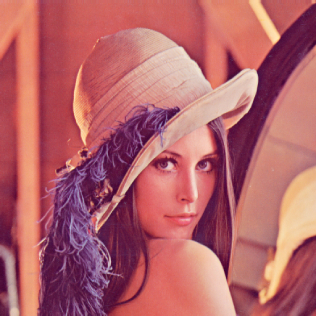
\includegraphics[width=.2\textwidth]{Lenna.jpg}
                    \caption{Lenna}
                    \label{Lenna}
                \end{figure}
                \item[(b)] As the subfigures \ref{lenna1} and \ref{lenna2} in \ref{Lenna2}.
                \begin{figure}[h]
                    \centering
                    \subfigure[lenna1]{
                    \label{lenna1}
                    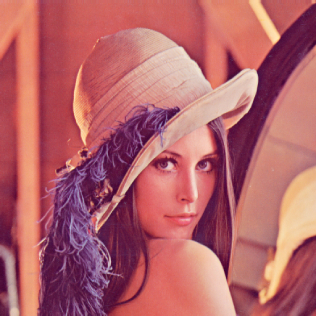
\includegraphics[width=.2\textwidth]{Lenna.jpg}}
                    \subfigure[lenna2]{
                    \label{lenna2}
                    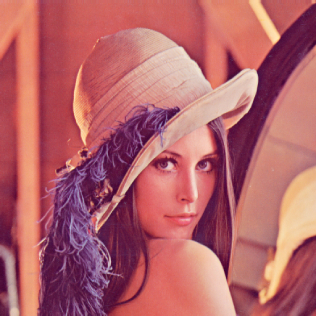
\includegraphics[width=.2\textwidth]{Lenna.jpg}}
                    \caption{Lenna2}
                    \label{Lenna2}
                \end{figure}
            \end{itemize}
            \item[(2)] As table \ref{my-table}.
            \begin{center}
                \begin{longtable}{ccccc}
                    \caption{Exemplary table}
                    \label{my-table}\\ \toprule
                    \multirow{2}{*}{\begin{tabular}[c]{@{}c@{}}merged multi-row\\ cell\end{tabular}} & \multicolumn{2}{c}{merged muti-column cell} & \multicolumn{2}{c}{merged muti-column cell} \\ \cline{2-5} 
                      & Column 1 & Column 2 & Column a & Column b \\ \midrule
                      If  & you    & shed & tears & when  \\
                      you & missed & the  & sun   &       \\
                      you & also   & miss & the   & stars \\ \bottomrule
                \end{longtable}
            \end{center}
            \item[(3)] Code are shown as following:
\begin{lstlisting}[language=Fortran]
program main
    implicit none

    write(*,*) 'hello world'
end program main
\end{lstlisting}
            \item[(4)] This book \cite{cohen2006quantum} provides a good introduction to quantum mechanics.
        \end{itemize}
    \end{sol}

    \bibliographystyle{unsrt}
    \bibliography{Assignment-en}
\end{document}